\documentclass{beamer}
\usepackage[utf8]{inputenc}
\usepackage{amsmath}
\usepackage{graphicx}
\graphicspath{{../images/}{../../shared/images/}}
\usepackage{xcolor}
\usepackage{tikz}

\usetheme{Madrid}
\usecolortheme{default}

% Define custom colors inspired by Star Trek DS9
\definecolor{ds9blue}{RGB}{25,25,112} % Midnight Blue
\definecolor{ds9gold}{RGB}{218,165,32} % Goldenrod
\definecolor{ds9grey}{RGB}{105,105,105} % Dim Gray
\definecolor{ds9red}{RGB}{178,34,34} % Firebrick

% Customize the colors
\setbeamercolor{title}{fg=ds9gold}
\setbeamercolor{frametitle}{bg=ds9blue, fg=white}
\setbeamercolor{block title}{bg=ds9gold, fg=black}
\setbeamercolor{block body}{bg=ds9grey!20, fg=black}
\setbeamercolor{section in toc}{fg=ds9gold}
\setbeamercolor{subsection in toc}{fg=ds9gold!70}
\setbeamercolor{footline}{bg=ds9blue, fg=white}
\setbeamercolor{author in head/foot}{fg=white}
\setbeamercolor{date in head/foot}{fg=white}
\setbeamercolor{title in head/foot}{fg=white}

% Title page configuration
\title[ Vector Analysis]{PHYS11 CH:5.1-5.3}
\subtitle{Vector Analysis and Applications }
\author[Mr. Gullo]{Mr. Gullo}
\date[Oct 2024]{October 2024}

% Table of contents at the beginning of each section
\AtBeginSection[]
{
  \begin{frame}
    \frametitle{Table of Contents}
    \tableofcontents[currentsection]
  \end{frame}
}

% Add logo
\logo{
\includegraphics[width=0.1\linewidth]{cinec_logo.png}}

\begin{document}

\frame{\titlepage}

\begin{frame}
\frametitle{Introduction to Vector Analysis}
\begin{itemize}
    \item Vectors are essential in physics for describing quantities with magnitude and direction
    \item Key topics:
    \begin{itemize}
        \item Vector addition and subtraction
        \item Resolving vectors into components
        \item Vector applications in real-world problems
    \end{itemize}
\end{itemize}
\end{frame}

\section{Vector Operations}

\begin{frame}
\frametitle{Trig Review}
\begin{columns}[T] % Top-aligned columns
    \column{0.48\textwidth}
    \begin{figure}
        \centering
        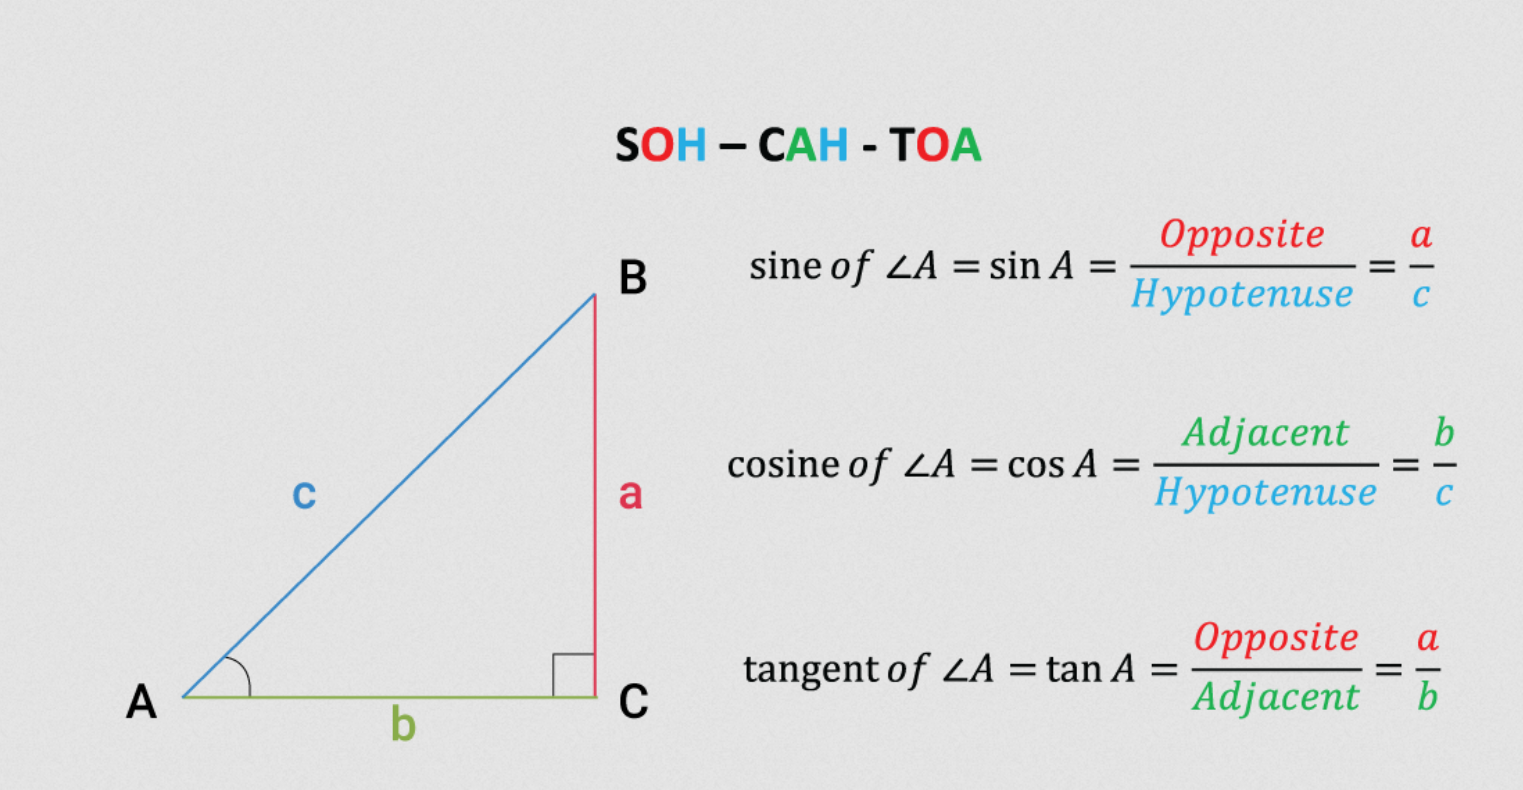
\includegraphics[width=\linewidth]{phys11-math-trigonometry-sohcahtoa.png}
        \caption{SOHCAHTOA mnemonic}
    \end{figure}

    \column{0.48\textwidth}
    \begin{figure}
        \centering
        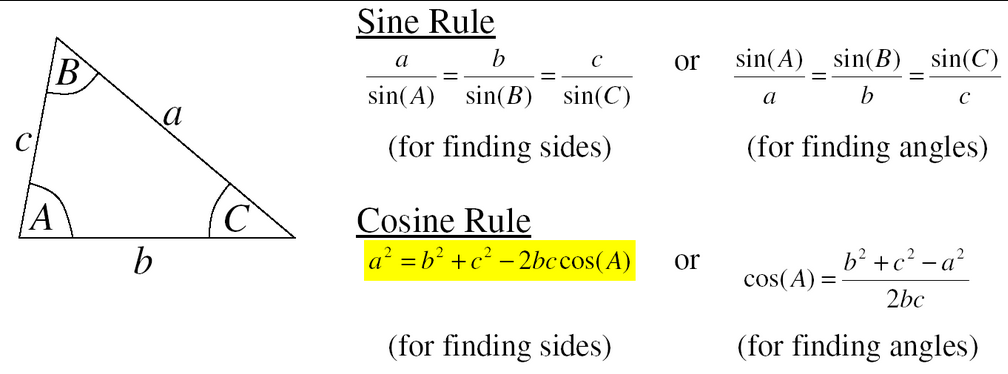
\includegraphics[width=\linewidth]{phys11-math-sine-cosine-laws.png}
        \caption{Sine and Cosine Laws}
    \end{figure}
\end{columns}
\end{frame}

\begin{frame}
\frametitle{Vector Addition and Subtraction}
\begin{itemize}
    \item Vector addition:
- Tip-to-tail method
- Parallelogram method

\item Vector subtraction:
- Add the negative of the vector: $\vec{A} - \vec{B} = \vec{A} + (-\vec{B})$

\item Resultant vector: $\vec{R} = \vec{A} + \vec{B}$
 \\
- For n vectors: $\vec{R} = \vec{A} + \vec{B} + \vec{C} + ... + \vec{N}$
\end{itemize}
\end{frame}

\begin{frame}
\frametitle{Vector Addition and Subtraction}
\begin{itemize}
\item Magnitude of resultant:\\
- General case: $|\vec{R}| = \sqrt{A^2 + B^2 + 2AB\cos\theta}$\\
- For perpendicular vectors: $|\vec{R}| = \sqrt{A^2 + B^2}$

\item Direction of resultant:\\
- Using magnitudes and angle: $\tan\phi = \frac{B\sin\theta}{A + B\cos\theta}$\\
- Using components: $\tan\phi = \frac{A_y + B_y}{A_x + B_x}$, 

\end{itemize}
\end{frame}

\begin{frame}
\frametitle{Resolving Vectors into Components}
\begin{itemize}
    \item Any vector can be resolved into x and y components
    \item $A_x = A\cos\theta$, $A_y = A\sin\theta$
    \item Magnitude: $A = \sqrt{A_x^2 + A_y^2}$
    \item Direction: $\tan\theta = \frac{A_y}{A_x}$
\end{itemize}
\end{frame}

\section{Vector Applications}

\begin{frame}
\frametitle{Example 1: River Crossing Problem}
Problem: A river flows SW to NE at 7.1 m/s. A boat moving at 13 m/s wants to reach a point due east.


\end{frame}
\begin{frame}
\frametitle{Example 1: River Crossing Problem}
Problem: A river flows SW to NE at 7.1 m/s. A boat moving at 13 m/s wants to reach a point due east.\\

Solution:
\begin{itemize}
    \item River velocity components: $v_{rx} = v_{ry} = 7.1\cos45° = 5.02$ m/s
    \item Boat must counteract river's y-component: $v_{by} = -5.02$ m/s
    \item Angle of boat's heading: $\theta = \arcsin(-5.02/13) \approx -22.6°$
\end{itemize}
Answer: The boat should head 22.6° south of east.
\end{frame}

\begin{frame}
\frametitle{Example 2: Displacement Problem}
Problem: A person walks 10.0 m north, then 2.0 m east. Find the resultant displacement.

\end{frame}

\begin{frame}
\frametitle{Example 2: Displacement Problem}
Problem: A person walks 10.0 m north, then 2.0 m east. Find the resultant displacement.

Solution:
\begin{itemize}
    \item Use Pythagorean theorem: $R = \sqrt{10.0^2 + 2.0^2} \approx 10.2$ m
    \item Angle: $\theta = \arctan(10.0/2.0) \approx 78.7°$ north of east
\end{itemize}
Answer: $\vec{R} = 10.2$ m, 78.7° north of east
\end{frame}
\section{Projectile Motion}

\begin{frame}
\frametitle{Projectile Motion Basics}
\begin{itemize}
    \item Combination of horizontal and vertical motion
    \item Horizontal motion: constant velocity (neglecting air resistance)
    \item Vertical motion: constant acceleration due to gravity
    \item Key equations:
    \begin{itemize}
        \item Range: $R = \frac{v_0^2 \sin(2\theta)}{g}$
        \item Maximum height: $h_{\max} = \frac{v_0^2 \sin^2\theta}{2g}$
        \item Time of flight: $t = \frac{2v_0 \sin\theta}{g}$
    \end{itemize}
\end{itemize}
\end{frame}

\begin{frame}
\frametitle{Example 3: Projectile Motion Problem}
Problem: A water-balloon cannon fires at 30 m/s, 50° above horizontal. Find the range.

\end{frame}
\begin{frame}
\frametitle{Example 3: Projectile Motion Problem}
Problem: A water-balloon cannon fires at 30 m/s, 50° above horizontal. Find the range.

Solution:
\begin{itemize}
    \item Use range equation: $R = \frac{v_0^2 \sin(2\theta)}{g}$
    \item $R = \frac{(30 \text{ m/s})^2 \sin(2 * 50°)}{9.8 \text{ m/s}^2} \approx 90.44$ m
\end{itemize}
Answer: The water balloon will fall approximately 90.44 m away.
\end{frame}
\begin{frame}
\frametitle{Conclusion}
\begin{itemize}
    \item Vector analysis is crucial for understanding motion in physics
    \item Key concepts covered:
    \begin{itemize}
        \item Vector addition and subtraction
        \item Resolving vectors into components
        \item Applications in real-world problems
        \item Basics of projectile motion
    \end{itemize}
    \item These concepts help analyze complex motions and solve practical problems
    \item Practice with various examples to master vector analysis
\end{itemize}
\end{frame}

\begin{frame}
\frametitle{Global Angles}

\begin{block}{Problem}
What is the global angle of 20° south of west?
\end{block}

\begin{center}
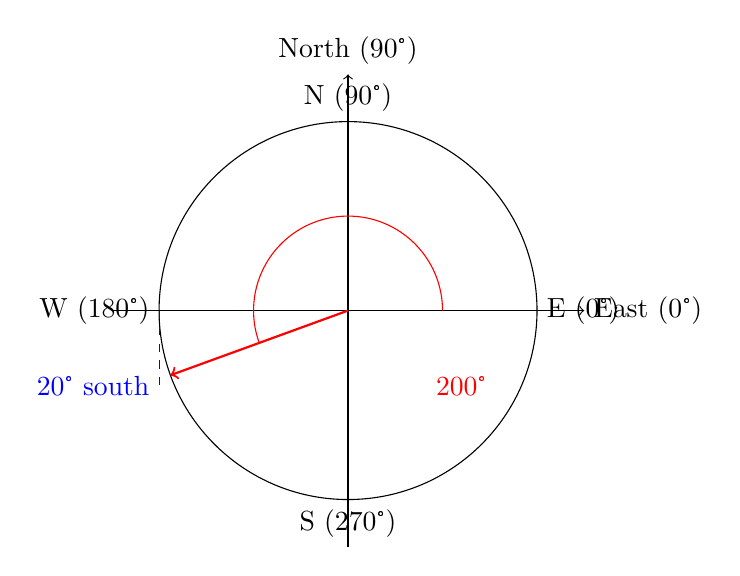
\begin{tikzpicture}[scale=1.2]
    % Draw main circle
    \draw (0,0) circle (2);
    
    % Draw axes
    \draw[->] (-2.5,0) -- (2.5,0) node[right] {East (0°)};
    \draw[->] (0,-2.5) -- (0,2.5) node[above] {North (90°)};
    
    % Draw compass directions
    \node[above] at (0,2) {N (90°)};
    \node[left] at (-2,0) {W (180°)};
    \node[right] at (2,0) {E (0°)};
    \node[below] at (0,-2) {S (270°)};
    
    % Draw the angle
    \draw[->, thick, red] (0,0) -- ({2*cos(200)}, {2*sin(200)});
    \draw[red] (1,0) arc (0:200:1);
    
    % Label the angle
    \node[red] at (1.2,-0.8) {200°};
    
    % Show the "south of west" reference
    \draw[blue, dashed] (-2,0) -- (-2,-0.8) node[left] {20° south};
    
\end{tikzpicture}
\end{center}
\end{frame}

\begin{frame}
\frametitle{River Crossing Problem}
\begin{block}{Problem}
A person attempts to cross a river in a straight line by navigating a boat at $15 \mathrm{~m} / \mathrm{s}$. If the river flows at $5.0 \mathrm{~m} / \mathrm{s}$ from left to right, what would be:
\begin{itemize}
    \item The magnitude of the boat's resultant velocity?
    \item The direction relative to the straight line across the river?
\end{itemize}
\end{block}

\begin{center}
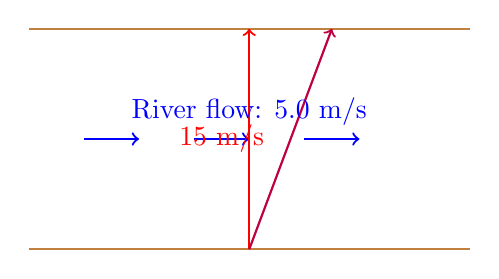
\begin{tikzpicture}[scale=0.7]
    % River banks
    \draw[thick, brown] (-4,2) -- (4,2);
    \draw[thick, brown] (-4,-2) -- (4,-2);
    
    % River flow arrows
    \draw[->, blue, thick] (-3,0) -- (-2,0);
    \draw[->, blue, thick] (-1,0) -- (0,0);
    \draw[->, blue, thick] (1,0) -- (2,0);
    
    % Boat's intended direction
    \draw[->, thick, red] (0,-2) -- (0,2);
    
    % Resultant motion
    \draw[->, thick, purple] (0,-2) -- (1.5,2);
    
    % Labels
    \node[blue] at (0,0.5) {River flow: $5.0 \mathrm{~m}/\mathrm{s}$};
    \node[red] at (-0.5,0) {$15 \mathrm{~m}/\mathrm{s}$};
\end{tikzpicture}
\end{center}

\end{frame}

\begin{frame}
\frametitle{River Crossing Solution}

The correct solution:
\begin{itemize}
    \item Resultant velocity: $15.8 \mathrm{~m} / \mathrm{s}$
    \item Direction: $18.4^{\circ}$ to the right
\end{itemize}


Using the Pythagorean theorem:
\[v_\text{resultant} = \sqrt{(5.0)^2 + (15.0)^2} = 15.8 \mathrm{~m}/\mathrm{s}\]

The angle is given by:
\[\theta = \tan^{-1}\left(\frac{5.0}{15.0}\right) = 18.4^\circ\]

\end{frame}

\end{document}